\documentclass[../main.tex]{subfiles}

\begin{document}
\section{구성}
본 교재는 파이썬 3의 문법과 알고리즘을 기초부터 익힐 수 있도록 구성되어 있습니다.
특히 파이썬의 기본적인 문법 숙지와 더불어 자주 사용되는 패턴에 익숙해지는 것에 초점을 맞추고 있습니다.
프로그래밍 언어를 처음 접하더라도 익힐 수 있도록 구성되어 있으나, 어느 정도의 수학적 배경 지식을 가정합니다.

또한, 정보과학적인 사고(순차적으로 논리적인 비약이 없이 문제 해결을 할 수 있는 능력)를 배우고 간단한 알고리즈믹 문제의 해결법을 배우는 것이 목적입니다.

기본적으로 알고리즘보다는 언어 자체의 문법과 활용에 초점을 맞춘 커리큘럼이므로, 알고리즘을 본격적으로 다루기 위해서는 자료 구조와 알고리즘에 대해서 깊게 다루는 서적을 읽어보시는 것을 추천드립니다.
Python과 같이 언어를 익히고 난 다음에는 알고리즘을 배우고 실제로 구현할 수 있는 준비가 되어 있을 것입니다.

알고리즘에 대해서 더 배우고 싶으시다면 흔히 CLRS라고 불리우는 \textit{Introduction to Algorithms 3/e (MIT Press, 2009)}를 추천드립니다.
혹시 더 깊은 이해를 원하신다면, 저도 아직 읽어보지는 못했지만 커누스 교수의 TAOCP로 불리우는 \textit{The Art of Computer Programming} 시리즈\footnote{커누스 교수가 1968년부터 집필을 시작해 현재는 4권의 일부분까지 완성되어 있으며, 현재 7권까지 계획이 되어 있습니다. 빌 게이츠는 본인이 훌륭한 프로그래머라고 생각하면 TAOCP를 읽어보고, 다 읽을 수 있다면 자신에게 이력서를 보내라고 하였습니다. 여담으로, 커누스 교수는 이 책의 조판을 위해서 본 교재를 위해서 사용된 \TeX을 개발하였습니다.}를 읽어보시면 됩니다.

\section{들어가기 전에}
Python은 문법이 단순하면서도 활용 가능성이 무궁무진한 언어입니다.
단순히 `정보과학'만을 위해서 Python을 배운다기보다는, 평생 활용할 수 있는 도구를 배우는 것입니다.
Python은 R이나 Matlab 등과 함께 학문적인 용도로도 쓰임이 많은 언어입니다.
특히 Matlab과 다르게 Python은 오픈 소스에 무료인데다가, 단순히 데이터 처리만을 위한 언어가 아닙니다.
NumPy와 Matplotlib 등의 패키지를 활용한다면 Matlab이나 Mathematica와 같은 상용 프로그래밍 언어가 할 수 있는 다양한 작업들을 대등하게 할 수 있기도 합니다.

실제로 저는 학업 중 물리학, 천문학, 화학, 생물학 등의 분야에서 데이터 분석 및 차트 제작을 위해 Python을 활용하거나, Raspberry Pi와 연동하여 다양한 센서를 사용해 프로젝트를 진행하는데에도 사용했습니다.
또한 Django 등의 프레임워크를 사용한다면 웹서버를 구축할 수도 있는데, YouTube, Dropbox, Facebook, Netflix, Google, Instagram, Spotify 등의 유명 사이트들이 Python을 활용하여 서비스를 제공하고 있습니다.
이처럼 Python은 배워두면 무궁무진한 방면에서 활용할 수 있는 가능성을 가지고 있는 언어입니다.

\section{Python이란?}
\begin{figure}[htbp]
  \centering
  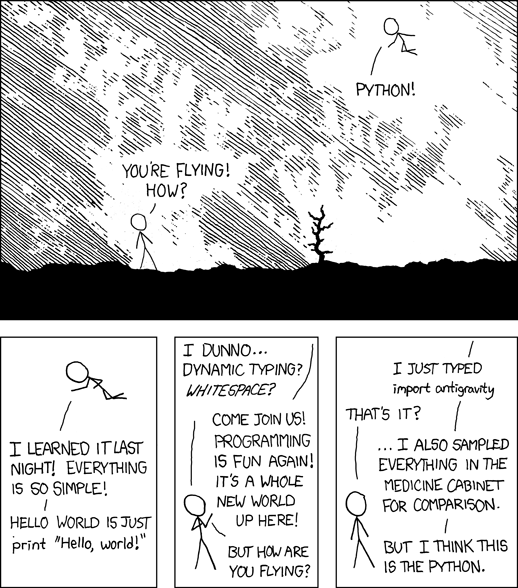
\includegraphics[width=0.6\linewidth]{./figures/xkcd_python}
  \caption*{흔히 Python을 ``batteries included''(배터리가 들어간) 언어라고 합니다.}\label{fig:meme}
\end{figure}
Python은 1991년에 Guido van Rossum이 발표한 프로그래밍 언어로, 문법이 굉장히 쉬우면서도 높은 생산성을 가지고 있는 언어입니다.\footnote{그가 1989년 크리스마스 연휴에 취미로 Python을 제작하였던 것이 그 시작입니다.}
특히 pseudocode의사코드와 유사하기 때문에 비교적 배우기 쉬워, 많은 학교에서 프로그래밍 입문 수업 언어로 Python을 채택하고 있습니다.
또, \textbf{프로그래밍 언어로 할 수 있을 법한 거의 모든 기능들이 이미 Python을 위한 패키지로 구현되어 있습니다.}
이 때문에 Python을 흔히 ``batteries included''라고 부릅니다.
따라서 속도가 중요한 작업이 아니라면 C/C++보다 Python을 쓰는 것이 효율적입니다.
(연산이 아니라 업무의 효율을 말하는 것입니다.)

프로그래밍에 익숙치 않더라도 컴퓨터에 관심이 많다면 C, C++, Java 등의 언어와 함께 Python도 한 번 쯤 들어보았을 정도로, Python은 점유율 상위 다섯 언어 안에 드는 주류 언어입니다.
Python은 1995년에 등장한 Java보다도 오래 전에 만들어진 언어로, 긴 역사를 가지고 있습니다.
그 만큼 버전의 숫자도 큰데, 이 글을 작성하는 현 시점에서 Python 2의 최신 버전은 2.7.16, Python 3의 최신 버전은 3.7.3입니다.
한동안은 Python 2와 Python 3가 동시에 개발되기도 하였고, Python 3보다는 Python 2를 사용하는 것이 낫다고 말하던 때가 있었습니다.\footnote{1, 2년 전까지만해도 Python 2 vs Python 3의 논쟁이 비일비재하게 일어났었습니다.}
그러나 현재는 Python 3를 배우고 사용하는 것이 권장됩니다.
Python 2는 2.7이 최종 버전이고, 이후에는 bugfix 릴리즈만 있을 예정인데다가 2020년까지만 지원을 할 예정입니다.
나아가 최신 버전의 Ubuntu(Linux 배포판의 한 버전)는 Python 3를 기본 Python 버전으로 설정하고 있습니다.

\textbf{Python은 interpreter인터프리터 언어입니다.}
Interpreter 언어란 소스 코드를 한 줄씩 기계어\footnote{기계가 바로 이해할 수 있는 저급 언어로, 0과 1의 이진수로만 구성되어 있는 언어로, 모든 CPU를 구동시키기 위해서는 C와 같은 고급 언어를 저급 언어로 변환시키는 과정이 필요합니다.}로 번역하는 방식의 언어입니다.
조금 더 가독성을 높인, 기계어와 일대일 대응이 되는 (마찬가지로 저급 언어인) 어셈블리어가 있기도 합니다.
고급 언어를 기계어로 변환시키는 방법은 크게 두 가지가 있습니다.
Compiler컴파일러와 interpreter입니다.
C와 같은 언어는 compiler 언어로, 코드 전체를 한꺼번에 기계어로 변환시킵니다.
이 때문에 실행 속도는 빠르다는 장점이 있지만, 코드를 수정하기 위해서는 다시 한 번 전체를 기계어로 변환시키는 과정이 필요합니다.
반면 Python은 한 줄씩 기계어로 번역하기 때문에 실행 속도는 다소 느리지만, debug디버그\footnote{코드에서 bug버그, 즉 오류를 제거하는 것을 의미합니다.}에 유리합니다.
한 줄씩 실행하기 때문에 애초에 compile을 거부하는 compiler 언어와는 다르게 버그가 있는 해당 줄까지 코드를 실행시켜주기 때문입니다.
이러한 장단점 때문에 프로그램의 골격을 Python으로 만들고, 빠른 연산이 필요한 부분만 C로 만드는 것도 가능합니다.

마지막으로, Python이 얼마나 쉽고 직관적인 언어인지 알아봅시다.
만약 A+가 F, C+, B0, A-, A+에 있으면 "A+가 있습니다."를 실행해주는 Python 코드를 봅시다.
\begin{minted}[mathescape,
               breaklines,
               numbersep=5pt,
               frame=lines,
               framesep=2mm]{python}
if "A+" in ["F", "C+", "B0", "A-", "A+"]: print("A+가 있습니다.")
\end{minted}
프로그래밍을 할 줄 모르더라도 저 코드를 이해할 수 있을 것입니다.
이처럼 Python은 인간이 사고하는 방식을 그대로 옮겨 놓았다고 해도 과언이 아닐만큼이나 직관적입니다.
익숙해진다면 자신이 하고 싶은 일을 코드로 옮기려고 끙끙댈 필요 없이, 생각하는 그대로 코드를 작성할 수 있을 것입니다.
참고로, 이와 같은 일을 하려면 C언어에서는 다음과 같이 해야 합니다.
\begin{minted}[mathescape,
               linenos,
               breaklines,
               numbersep=5pt,
               frame=lines,
               framesep=2mm]{c}
#include <stdio.h>
#include <string.h>
int main(void) {
    char grades[][3] = {"F", "C+", "B0", "A-", "A+"};
    for (int i = 0; i < 5; ++i) {
        if (strncmp(grades[i], "A+", 2) == 0) {
            printf("A+가 있습니다.\n");
        }
    }
    return 0;
}
\end{minted}
단 한 줄의 Python 코드로 될 일을 C 언어로는 10줄 이상으로 작성해야 하는 것입니다.
\end{document}
